\documentclass[11pt,a4paper]{article}
\usepackage[margin=2.3cm]{geometry}
\usepackage[T1]{fontenc}
\usepackage{lmodern,microtype,booktabs,array,pgfplots,xcolor,caption,enumitem}
\usepackage[hidelinks]{hyperref}
\pgfplotsset{compat=1.16}
\captionsetup{font=small,labelfont=bf}
\setlist{itemsep=2pt,topsep=3pt}
\title{Retrieval-Augmented Generation over the D\&D SRD:\\Deduplication, Hierarchical Routing, Hybrid Search, Graph RAG and Agentic RAG}
\author{}
\date{}
\begin{document}
\maketitle

\section{Summary}
We rebuilt the D\&D 5e SRD RAG pipeline for the full corpus (13 files, 5{,}200 chunks) and compared eight variants on 24 hard questions with a weak generator (Claude Haiku, called through isolated \texttt{claude -p}), with retrieval-only metrics (MRR, recall, nDCG), 41 open questions, and a replication with Qwen2.5-7B. To stop the model answering from memory of the published SRD, the index is built on a \emph{counterfactual} copy of the data in which 22 of 106 gold facts were changed.
\begin{itemize}
\item \textbf{The original duplication bug was the largest problem.} Each chunk was stored about four times, so 73\% of top-10 slots were exact copies and the cross-encoder only re-ordered copies. After deduplication the top-10 contains distinct chunks only.
\item \textbf{Ranking (semantic judge, fact accuracy):} agentic 98.6\% $>$ graph 86.7\% $>$ rerank-8 70.7\% $\approx$ hybrid 69.5\% $>$ baseline 58.6\% $\approx$ rerank-3 57.9\% $=$ hierarchical 57.9\% $>$ closed-book 51.7\%.
\item \textbf{Memory is real but removed by the design.} Closed-book Haiku gets 4.5\% of the changed facts but 64.3\% of the unchanged ones, so the unchanged facts alone would have hidden retrieval quality.
\item \textbf{What did not help:} hierarchical routing (same top-3 as flat search on 20 of 24 questions and the same score on all 24), BM25 hybrid fusion (no gain over simply reranking 8 dense chunks), and cross-encoder reranking of only 3 chunks (no gain over baseline). Most of the early ``improvement'' of larger pipelines is the larger context window.
\item \textbf{Verdict.} \textbf{Graph RAG is the best value:} the best retrieval quality of all variants (MRR 0.93, nDCG@8 56.1\%, recall@8 88.3\%), near-top answer accuracy, and only one LLM call. \textbf{Agentic RAG is the most accurate} on the Haiku run (98.6\%) but costs three calls and about three times the latency, and on the weaker Qwen generator it ties graph (Section~8). Hierarchical routing gives no benefit at this scale; reranking improves ranking (MRR 0.76 $\to$ 0.92) but not answers unless the context is also enlarged.
\item \textbf{What helped:} entity-linked graph expansion (+16 points over rerank-8) and agentic query decomposition with a sufficiency check (+12 points over graph, at 3 LLM calls per question).
\end{itemize}

\section{Fixing the index first: deduplication}
In the saved results of the original run, 73\% of top-10 slots were exact duplicates, and a typical query returned only 2--3 distinct chunks (the same chunk appeared about four times, with identical cosine scores). The source files had no such duplication; the vector store had been filled several times. Consequently the cross-encoder compared copies of the same text, and re-ranking could not change the answer.

Fixes, applied at index time and at query time:
\begin{itemize}
\item \textbf{Index time.} Every file in \texttt{data/} is split by Markdown header and then into 500-character chunks (50 overlap). Each chunk is prefixed with its section path (for example \texttt{[Spells > Fireball]}). The chunk id is the SHA-1 of the normalised section and text, which is also the ChromaDB id, so re-ingesting cannot create copies; an assertion checks that the store count equals the number of unique chunks (5{,}273 raw, 5{,}200 unique). The section path uses only the top-level title and the deepest header, because \texttt{spells.md} contains a stray \texttt{\#\# Otherworldly Steed} heading that otherwise became a wrong parent of every later spell.
\item \textbf{Query time.} Retrieval over-fetches 50 candidates and drops any chunk with cosine similarity $\ge 0.95$ to a higher-ranked kept chunk. On the earlier 27-question set, 270 of 270 top-10 chunks were distinct afterwards.
\end{itemize}

\section{Experimental setup}
\paragraph{Corpus and counterfactual copy.} The 13 SRD files in \texttt{data/} (about 1.9\,MB). \texttt{build\_cf.py} writes \texttt{data\_cf/} with 27 scoped edits, each asserted to land inside its target section, for example Fireball 8d6$\to$9d6 and 150$\to$120 feet, Counterspell's save Constitution$\to$Wisdom, Bag of Holding 500$\to$800 pounds, Owlbear AC 13$\to$15, the Soldier background's skills, the death-save threshold 10$\to$12, and the point-buy budget 27$\to$30. A model answering from memory gets these facts wrong; only correct retrieval gets them right.

\paragraph{Questions.} 24 questions in five types: multi-part (8), cross-file (6), needle (4), reasoning (2), multi-topic (4). Many ask for several things at once (up to seven facts per question, and up to four unrelated topics). Every gold fact (106 in total) is checked by script to occur in the counterfactual data (one derived fact, ``11d6'', excepted).

\paragraph{Generator and isolation.} Every LLM call (answers, the agentic planner, and the judge) uses \texttt{claude -p --model haiku} from an empty temporary directory with \texttt{--tools ""}, no session persistence, no setting sources, slash commands disabled, no MCP servers, and a minimal system prompt, so the model sees only the prompt text and cannot read the data folder. A direct probe confirmed it has no tools and no knowledge of the project files. The answer prompt tells the model that the context may differ from the official rules and is always right.

\paragraph{Scoring.} \emph{Fact accuracy} is the fraction of a question's gold facts that the answer states. The primary metric is a semantic check by Haiku (wording and formatting may differ; every number and name must match). A strict string-match metric is reported in the appendix because the judge shares the generator's model family. \emph{Full answer} means all facts stated. \emph{Context recall} is the fraction of gold facts present verbatim in the retrieved context, which separates retrieval quality from generation quality.

\section{Variants}
\begin{description}[leftmargin=1.2cm,labelwidth=1cm]
\item[V0] Closed-book control: the question alone, no context.
\item[V1] Dense search (all-MiniLM-L6-v2, ChromaDB with its HNSW index, cosine), near-duplicates removed, top-3 chunks.
\item[V2] V1's top-10 re-scored by the cross-encoder (ms-marco-MiniLM-L-6-v2), top-3.
\item[V2b] Same as V2 but top-8 chunks. This control isolates the effect of a larger context from the effect of any better method.
\item[V3] Hierarchical coarse-to-fine routing: score file centroids and discard half the files, keep the best 150 sections among the rest, search chunks only inside them (metadata filter), then rerank, top-3. HNSW is the index underneath every variant; routing is a separate layer on top of it.
\item[V4] Hybrid: dense search inside the routed space plus BM25 over all chunks, merged by reciprocal rank fusion, cross-encoder rerank, top-8.
\item[V5] Graph RAG (lightweight, no LLM extraction): nodes are section entities (1{,}706 spells, monsters, items, rules, \dots), an edge A$\to$B means a chunk of A mentions B (6{,}867 edges, 47 over-connected hub entities ignored). Entities named in the question contribute their best chunks directly; entities mentioned inside the top seed chunks are expanded one hop; the pooled candidates are reranked, top-8.
\item[V6] Agentic RAG: Haiku splits the question into at most six keyword queries; each is retrieved with the V4 pipeline (top-3 each); Haiku then lists missing facts, which trigger one follow-up retrieval round; Haiku answers from at most 16 chunks. Three LLM calls per question (planner, checker, answer).
\end{description}

\section{Results}
\begin{table}[h]\centering\footnotesize\setlength{\tabcolsep}{3.5pt}
\caption{Main results, ranked by semantic-judge fact accuracy (24 questions, 106 gold facts, one run each). ``Changed'' and ``unchanged'' split the facts by whether the counterfactual edit touched them.}
\begin{tabular}{@{}p{4.9cm}rrrrrrr@{}}\toprule
Variant & Fact acc. & Full ans. & Changed & Unch. & Ctx.\ rec. & Ctx.\ chars & LLM calls\\\midrule
V6 Agentic RAG (plan, retrieve, check, answer) & 98.6\% & 95.8\% & 100.0\% & 98.8\% & 99.0\% & 4291 & 3.0 \\
V5 Graph RAG (entity-linked), top-8 & 86.7\% & 66.7\% & 86.4\% & 86.9\% & 88.6\% & 3022 & 1.0 \\
V2b Rerank, top-8 (context control) & 70.7\% & 54.2\% & 63.6\% & 71.4\% & 75.2\% & 2688 & 1.0 \\
V4 Hybrid BM25+dense (RRF) + routing + rerank, top-8 & 69.5\% & 50.0\% & 59.1\% & 71.4\% & 80.0\% & 3026 & 1.0 \\
V1 Baseline dense (HNSW), top-3 & 58.6\% & 20.8\% & 54.5\% & 58.3\% & 57.1\% & 1041 & 1.0 \\
V2 + cross-encoder rerank, top-3 & 57.9\% & 20.8\% & 50.0\% & 58.3\% & 58.1\% & 1117 & 1.0 \\
V3 Hierarchical routing + rerank, top-3 & 57.9\% & 20.8\% & 50.0\% & 58.3\% & 58.1\% & 1131 & 1.0 \\
V0 Closed-book (no retrieval) & 51.7\% & 8.3\% & 4.5\% & 64.3\% & 0.0\% & 0 & 1.0 \\
\bottomrule\end{tabular}
\end{table}

\begin{figure}[h]\centering
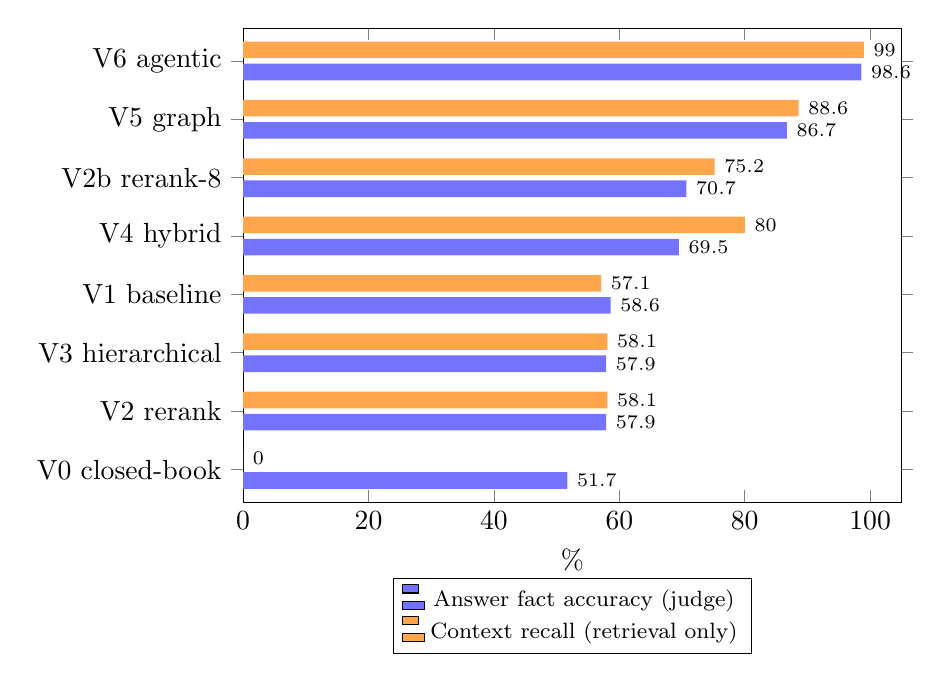
\begin{tikzpicture}
\begin{axis}[xbar,width=0.82\linewidth,height=7.6cm,xmin=0,xmax=105,bar width=6pt,symbolic y coords={V0 closed-book,V2 rerank,V3 hierarchical,V1 baseline,V4 hybrid,V2b rerank-8,V5 graph,V6 agentic},ytick=data,
 xlabel={\%},legend style={at={(0.5,-0.16)},anchor=north,legend columns=1,font=\footnotesize},enlarge y limits=0.08,nodes near coords,nodes near coords style={font=\scriptsize}]
\addplot[fill=blue!55,draw=none] coordinates {
(51.7,V0 closed-book)
(57.9,V2 rerank)
(57.9,V3 hierarchical)
(58.6,V1 baseline)
(69.5,V4 hybrid)
(70.7,V2b rerank-8)
(86.7,V5 graph)
(98.6,V6 agentic)
};
\addplot[fill=orange!70,draw=none] coordinates {
(0.0,V0 closed-book)
(58.1,V2 rerank)
(58.1,V3 hierarchical)
(57.1,V1 baseline)
(80.0,V4 hybrid)
(75.2,V2b rerank-8)
(88.6,V5 graph)
(99.0,V6 agentic)
};
\legend{Answer fact accuracy (judge),Context recall (retrieval only)}
\end{axis}
\end{tikzpicture}
\caption{Answer accuracy versus the share of gold facts that retrieval put into the context.}
\end{figure}

\begin{table}[h]\centering\small
\caption{Fact accuracy (judge) by question type; question counts: multi-part (8), cross-file (6), needle (4), reasoning (2), multi-topic (4).}
\begin{tabular}{@{}lrrrrr@{}}\toprule
Variant & multi-part & cross-file & needle & reasoning & multi-topic\\\midrule
V6 agentic & 100.0\% & 100.0\% & 100.0\% & 100.0\% & 91.7\% \\
V5 graph & 100.0\% & 89.1\% & 100.0\% & 87.5\% & 42.5\% \\
V2b rerank-8 & 88.8\% & 65.9\% & 87.5\% & 87.5\% & 16.7\% \\
V4 hybrid & 87.5\% & 63.3\% & 90.0\% & 62.5\% & 25.8\% \\
V1 baseline & 77.5\% & 50.9\% & 71.2\% & 87.5\% & 5.0\% \\
V2 rerank & 72.1\% & 59.2\% & 66.2\% & 62.5\% & 16.7\% \\
V3 hierarchical & 72.1\% & 59.2\% & 66.2\% & 62.5\% & 16.7\% \\
V0 closed-book & 66.9\% & 43.4\% & 72.9\% & 50.0\% & 13.3\% \\
\bottomrule\end{tabular}
\end{table}

\begin{table}[h]\centering\small
\caption{Paired differences in per-question fact accuracy (percentage points) with 95\% bootstrap intervals over the 24 questions (10{,}000 resamples).}
\begin{tabular}{@{}lrr@{}}\toprule
Comparison & Mean difference & 95\% interval\\\midrule
Agentic vs.\ graph & +12.0 & [+4.7, +20.5] \\
Graph vs.\ rerank-8 & +16.0 & [+6.8, +25.9] \\
Hybrid vs.\ rerank-8 & -1.2 & [-14.3, +11.4] \\
Rerank-8 vs.\ rerank-3 & +12.8 & [+4.6, +22.8] \\
Rerank-3 vs.\ baseline & -0.7 & [-11.4, +9.3] \\
Hierarchical vs.\ rerank-3 & +0.0 & [+0.0, +0.0] \\
\bottomrule\end{tabular}
\end{table}

\section{Retrieval-only metrics}
Answer accuracy mixes retrieval and generation. To rank the retrievers alone we need no LLM: a chunk is \emph{relevant} to a question if it contains at least one of its gold facts (string match in the counterfactual corpus), and its gain is the number of distinct gold facts it contains. The ranked list is the list of chunks that was sent to the generator, in the order it was sent. We report \textbf{MRR} (reciprocal rank of the first relevant chunk), \textbf{Hit@$k$}, \textbf{Recall@$k$} (share of gold facts covered by the top $k$), \textbf{Precision@$k$}, \textbf{nDCG@$k$} (graded gain, normalised by the best possible ranking over all 5{,}200 chunks) and \textbf{Full@$k$} (all gold facts covered). Retrieval does not depend on the generator, so these numbers hold for any model.

\begin{table}[h]\centering\footnotesize\setlength{\tabcolsep}{3pt}
\caption{Retrieval quality of the chunks sent to the LLM (24 questions), ranked by nDCG@8. Variants with 3 chunks send fewer than 8, so their @8 values equal their @3 values by construction. $^\dagger$Agentic chunks come from several sub-queries concatenated, so MRR and nDCG are not meaningful for its order; its recall is.}
\resizebox{\linewidth}{!}{\begin{tabular}{@{}lrrrrrrrrr@{}}\toprule
Variant & Chunks & MRR & Hit@3 & Rec@3 & nDCG@3 & Rec@8 & Prec@8 & nDCG@8 & Full@8\\\midrule
V5 graph & 8.0 & 0.931 & 100.0\% & 70.3\% & 66.3\% & 88.3\% & 47.4\% & 56.1\% & 70.8\% \\
V4 hybrid & 8.0 & 0.931 & 100.0\% & 64.9\% & 62.0\% & 80.5\% & 43.2\% & 52.0\% & 58.3\% \\
V2b rerank-8 & 8.0 & 0.917 & 91.7\% & 61.3\% & 61.8\% & 75.8\% & 40.6\% & 50.8\% & 62.5\% \\
V6 agentic & 11.3 & 0.842$^\dagger$ & 91.7\% & 41.5\% & 40.7\%$^\dagger$ & 85.0\% & 41.5\% & 45.4\%$^\dagger$ & 62.5\% \\
V3 hierarchical & 3.0 & 0.917 & 91.7\% & 61.3\% & 62.1\% & 61.3\% & 65.3\% & 42.3\% & 25.0\% \\
V2 rerank & 3.0 & 0.917 & 91.7\% & 61.3\% & 61.8\% & 61.3\% & 65.3\% & 42.1\% & 25.0\% \\
V1 baseline & 3.0 & 0.750 & 83.3\% & 58.6\% & 51.3\% & 58.6\% & 58.3\% & 35.7\% & 25.0\% \\
\bottomrule\end{tabular}}
\end{table}

\begin{table}[h]\centering\footnotesize
\caption{Candidate pool seen by the cross-encoder, and ranking quality before and after re-ranking. ``Pool recall'' is the share of gold facts present anywhere in the pool.}
\begin{tabular}{@{}lrrrrrr@{}}\toprule
Variant & Pool size & Pool recall & MRR before & MRR after & nDCG@8 before & nDCG@8 after\\\midrule
V2 rerank & 10 & 74.5\% & 0.764 & 0.917 & 44.5\% & 50.1\% \\
V2b rerank-8 & 10 & 74.5\% & 0.764 & 0.917 & 44.5\% & 50.1\% \\
V3 hierarchical & 10 & 74.5\% & 0.777 & 0.917 & 45.0\% & 50.7\% \\
V4 hybrid & 30 & 86.6\% & 0.859 & 0.931 & 51.2\% & 52.4\% \\
V5 graph & 20 & 94.3\% & 0.859 & 0.931 & 51.2\% & 55.8\% \\
V6 agentic & 20 & 57.7\% & 0.695 & 0.826 & 29.2\% & 33.5\% \\
\bottomrule\end{tabular}
\end{table}

\begin{itemize}
\item \textbf{Graph RAG retrieves best.} It has the highest MRR (tied with hybrid), the highest recall at 3 and at 8, the highest precision@3, the highest nDCG at 3 and 8 and full-coverage rate, and the largest candidate pool recall (94\%). Entity linking puts the sections the question names into the pool, which similarity search alone often misses.
\item \textbf{The cross-encoder is what makes ranking good.} On the same pool, re-ranking raises MRR from about 0.76 to 0.92. Baseline top-3 (no reranker) has MRR 0.75; with the reranker it is 0.92.
\item \textbf{Routing does not change retrieval.} Hierarchical and flat search have the same pool recall (74.5\%) and the same MRR after re-ranking; routing only changes where the search looks, not what the reranker keeps.
\item \textbf{Three chunks are not enough.} Full@8 is 25\% for all top-3 variants: for three out of four questions the context lacks at least one gold fact. Eight chunks lift it to 58--71\%.
\item \textbf{Agentic covers the most facts per question but ranks worse} (Recall@8 85\%, but MRR 0.84), because it concatenates sub-query results; the first chunk is the best chunk of the first sub-query, not of the whole question.
\end{itemize}

\section{Open-ended questions (no gold answers)}
We also ran all variants on 41 open questions written by an LLM (characters, spells, classes, monsters, equipment) over the \emph{original} SRD. They have no gold answers, so the evaluation uses several different measures, each by an isolated Haiku judge unless marked automatic: \textbf{faithfulness} (share of claims in the answer supported by the retrieved context), \textbf{completeness} (0--2, scaled; ``the information is not available'' counts as 0), \textbf{context precision} (share of retrieved chunks relevant to the question), \textbf{entity hit} (automatic: share of entities named in the question whose section appears in the context), and \textbf{abstention} (automatic: the answer says the context lacks the information). Two questions cannot be answered from the SRD (Beholder, Mind Flayer); a good system abstains on them and not on the rest.

\begin{table}[h]\centering\footnotesize
\caption{Open-question metrics (41 questions, Haiku generator and judge). ``Abst.\ ans.'' is the abstention rate on answerable questions (lower is better); ``Abst.\ unans.'' is the rate on the two unanswerable ones (higher is better).}
\begin{tabular}{@{}lrrrrrrrr@{}}\toprule
Variant & Faithful & Complete & Ctx prec. & Entity hit & Abst.\ ans. & Abst.\ unans. & LLM calls & Sec/q\\\midrule
V6 agentic & 95.7\% & 56.1\% & 41.6\% & 71.4\% & 64.9\% & 100.0\% & 3.0 & 18.5 \\
V5 graph & 95.1\% & 52.4\% & 41.8\% & 76.8\% & 51.4\% & 100.0\% & 1.0 & 6.6 \\
V4 hybrid & 94.2\% & 54.9\% & 47.0\% & 71.4\% & 56.8\% & 100.0\% & 1.0 & 8.7 \\
V2b rerank-8 & 92.6\% & 48.8\% & 42.4\% & 67.9\% & 59.5\% & 100.0\% & 1.0 & 7.5 \\
V2 rerank & 97.6\% & 40.2\% & 61.0\% & 50.0\% & 70.3\% & 100.0\% & 1.0 & 5.8 \\
V3 hierarchical & 95.6\% & 36.6\% & 60.2\% & 50.0\% & 73.0\% & 100.0\% & 1.0 & 5.4 \\
V1 baseline & 95.0\% & 37.8\% & 56.9\% & 51.8\% & 62.2\% & 100.0\% & 1.0 & 5.5 \\
\bottomrule\end{tabular}
\end{table}

\begin{itemize}
\item \textbf{Faithfulness is high everywhere (93--98\%)}, so none of the RAG variants hallucinates much beyond its context. The top-3 variants are the most faithful, simply because they have less to misread.
\item \textbf{Chunk-level retrieval over-abstains on broad questions.} Between 51\% and 73\% of answerable questions are answered with ``the context does not say'' because the answer is spread over a whole section (for example, a class's full feature list). Graph RAG abstains least (51\%) and has the best entity hit rate (77\%); hierarchical and rerank-3 abstain most (70--73\%). This is the main weakness left, and it points to section-level (parent-document) retrieval as the next step.
\item \textbf{Precision and recall trade off.} Top-3 variants have the highest context precision (57--61\%) and lowest completeness (37--40\%); the 8-chunk variants and agentic invert this.
\item \textbf{Closed-book looks best here, which is the contamination problem again.} On unmodified SRD text a model that has read the SRD answers 85\% correctly without retrieval, but it never abstains, so it also fabricates on the two unanswerable questions (0\% abstention versus 100\% for every RAG variant except graph in the Qwen run). A correctness-versus-reference score was computed but is reliable for only 13 of the 41 questions (entity linking found the reference sections only there), so we do not use it for ranking.
\end{itemize}

\section{Replication with a small open model (Qwen2.5-7B-Instruct)}
To check that the ranking is not an artefact of one proprietary generator, we repeated both experiments with Qwen2.5-7B-Instruct (4-bit, one T4 GPU on Colab), keeping the retrieval, prompts and questions identical; retrieval was replayed to store the chunk rankings, and its candidate lists are the same as in Section~6. Qwen judging its own kind was unusable (it scored closed-book answers 96\% correct), so Qwen's answers were scored by the same Haiku judge and by the strict string match.

\begin{table}[h]\centering\footnotesize
\caption{Haiku and Qwen as generators (24 counterfactual questions; open-question abstention). ``Judge'' is the Haiku semantic judge, ``strict'' the string match. Spearman rank correlation between the Haiku and Qwen rankings: 0.97 (judge) and 0.87 (strict).}
\resizebox{\linewidth}{!}{\begin{tabular}{@{}lrrrrrrr@{}}\toprule
Variant & Haiku judge & Qwen judge & Qwen changed facts & Haiku strict & Qwen strict & Qwen abst.\ ans. & Qwen abst.\ unans.\\\midrule
V6 agentic & 98.6\% & 84.3\% & 77.3\% & 84.3\% & 65.0\% & 48.6\% & 100\% \\
V5 graph & 86.7\% & 81.9\% & 81.8\% & 76.0\% & 66.1\% & 40.5\% & 50\% \\
V4 hybrid & 69.5\% & 68.7\% & 68.2\% & 67.1\% & 56.7\% & 43.2\% & 100\% \\
V2b rerank-8 & 70.7\% & 61.8\% & 50.0\% & 66.2\% & 59.4\% & 35.1\% & 100\% \\
V1 baseline & 58.6\% & 51.9\% & 50.0\% & 51.2\% & 48.5\% & 48.6\% & 100\% \\
V3 hierarchical & 57.9\% & 49.4\% & 36.4\% & 52.0\% & 40.9\% & 43.2\% & 100\% \\
V2 rerank & 57.9\% & 47.3\% & 36.4\% & 52.6\% & 40.9\% & 45.9\% & 100\% \\
V0 closed-book & 51.7\% & 33.0\% & 4.5\% & 37.2\% & 21.3\% & 0.0\% & 0\% \\
\bottomrule\end{tabular}}
\end{table}

\begin{table}[h]\centering\footnotesize
\caption{Open-question metrics with Qwen as generator (41 questions; Haiku judge). ``Correct'' is the score against the oracle reference and is defined for 13 questions only.}
\begin{tabular}{@{}lrrrrrrr@{}}\toprule
Variant & Faithful & Complete & Ctx prec. & Entity hit & Correct & Abst.\ ans. & Abst.\ unans.\\\midrule
V6 agentic & 84.3\% & 40.2\% & 47.5\% & 57.1\% & 53.8\% & 48.6\% & 100.0\% \\
V5 graph & 81.6\% & 50.0\% & 44.8\% & 76.8\% & 61.5\% & 40.5\% & 50.0\% \\
V4 hybrid & 85.9\% & 45.1\% & 45.4\% & 71.4\% & 53.8\% & 43.2\% & 100.0\% \\
V2b rerank-8 & 81.0\% & 50.0\% & 42.7\% & 67.9\% & 61.5\% & 35.1\% & 100.0\% \\
V2 rerank & 83.1\% & 35.4\% & 63.4\% & 50.0\% & 50.0\% & 45.9\% & 100.0\% \\
V3 hierarchical & 86.9\% & 41.5\% & 60.2\% & 50.0\% & 42.3\% & 43.2\% & 100.0\% \\
V1 baseline & 80.0\% & 39.0\% & 59.3\% & 51.8\% & 50.0\% & 48.6\% & 100.0\% \\
V0 closed-book & -- & 76.8\% & -- & -- & 15.4\% & 0.0\% & 0.0\% \\
\bottomrule\end{tabular}
\end{table}

\begin{itemize}
\item \textbf{The ranking transfers.} Agentic and graph are the top two with both generators, the 8-chunk variants follow, then baseline and the 3-chunk rerankers, and closed-book is last, getting only 4.5\% of the changed facts. Rank correlation with Haiku is 0.97.
\item \textbf{With the weaker generator the gap between graph and agentic closes.} The judge puts agentic ahead by about 2 points (84\% vs.\ 82\%) and the string metric puts graph ahead by about 1 point; neither difference is meaningful at 24 questions, so the two extra LLM calls of agentic RAG buy little here.
\item \textbf{Qwen is less faithful than Haiku} (80--87\% of claims supported by context, versus 93--98\%), so a stronger generator matters even with good retrieval.
\item \textbf{Qwen shows the value of retrieval on the open questions.} Qwen has not memorised the SRD: closed-book Qwen is correct on 15\% of the answerable reference questions, against 85\% for Haiku, while the RAG variants reach 42--62\%. Rerank-8 and graph score best (62\%), on the 13 questions that have a reference.
\item \textbf{Abstention.} Qwen abstains less than Haiku on answerable questions (35--49\% versus 51--73\%); rerank-8 abstains least. Graph is the only variant that failed to abstain on one of the two unanswerable questions.
\end{itemize}

\section{Discussion}
\paragraph{The counterfactual design matters.} Closed-book Haiku scores 64.3\% on unchanged facts, close to what several RAG variants reach overall, and 4.5\% on changed facts. On unmodified data alone, V1--V3 would look only a few points better than no retrieval. The ranking among retrieval methods is cleanest in the ``changed'' column.

\paragraph{Retrieval quality gates everything.} Answer accuracy tracks context recall closely (Figure~1). V1--V3 retrieve only 3 chunks and miss about 40\% of the needed facts; questions that need several entities (multi-topic) are almost unanswerable for them.

\paragraph{Hierarchical routing: no benefit here.} V3 returned the same top-3 as V2 on 20 of the 24 questions and scored identically on all 24 (difference exactly 0). Routing did not discard chunks that mattered, so it is safe, but at 5{,}200 chunks plain HNSW is already fast and accurate; on the earlier spell-only set the routed search was also slower per query (about 23\,ms vs.\ 8\,ms). It may pay off at much larger scale or with many unrelated files, which our questions only partly exercise.

\paragraph{Hybrid search: no gain beyond context size.} V4 reaches higher context recall than V2b (80\% vs.\ 75\%) but not higher answer accuracy, and the difference is within noise. Adding BM25 and routing did not beat reranking 8 dense chunks.

\paragraph{Graph RAG helps most on multi-entity questions.} Linking entities named in the question to their own sections guarantees that each named spell, monster or item contributes a chunk, which plain similarity search does not. V5 gains 16 points over rerank-8 with the same context size and one LLM call, and its extra cost is an offline graph build over the chunks. It still struggles on multi-topic questions with up to four unrelated parts (42.5\% accuracy in Table~2): several of the facts for the later parts never reach its context.

\paragraph{Agentic RAG is best but costs more.} Splitting the question into focused queries (on average 4.3 per question) and checking for missing facts gives the highest context recall (99.0\%) and the best answers, including the multi-topic questions. It needs three LLM calls and was the slowest variant (about 15\,s per question versus about 6\,s, measured with four calls in parallel). The checker requested follow-up retrieval on 33.3\% of questions. It also passed the largest context (about 4291 characters).

\section{Which system is better?}
\begin{table}[h]\centering\small
\caption{Best system per criterion.}
\begin{tabular}{@{}p{5.6cm}p{3.1cm}p{6.2cm}@{}}\toprule
Criterion & Winner & Evidence\\\midrule
Answer accuracy, Haiku (judge) & Agentic (98.6\%) & +12 points over graph; wider interval, see Table~3\\
Answer accuracy, Qwen & Agentic $\approx$ graph & judge 84\% vs.\ 82\%; strict 65\% vs.\ 66\%; within noise\\
Ranking quality (MRR, nDCG) & Graph, hybrid & MRR 0.93; graph best nDCG@3 and nDCG@8\\
Coverage of gold facts (Rec@8, pool) & Graph, then agentic & 88\% and 85\% at 8 chunks; pool recall 94\%\\
Fewest LLM calls for the accuracy & Graph & one call; agentic uses three\\
Fewest unanswered answerable questions & Graph & 51\% abstention vs.\ 57--73\% for others\\
Faithfulness, context precision & Rerank top-3 & fewest chunks, least to misread (but least complete)\\
Latency and simplicity & Baseline & single dense search; no gain in accuracy\\
\bottomrule\end{tabular}
\end{table}

\paragraph{Overall.} \textbf{Graph RAG is the best system for this corpus}: it is first or tied for first on MRR, nDCG, recall and full coverage, close to the top on answers with both generators, and costs one LLM call. \textbf{Agentic RAG is the choice when maximum accuracy matters and three LLM calls are affordable}, and it helps most with a strong generator. \textbf{Hybrid search and larger context (rerank-8)} are the cheap middle ground. \textbf{Hierarchical routing and a 3-chunk reranker add complexity without improving answers}; the cross-encoder is worth keeping only if the context is also widened. Deduplication, not any of the advanced methods, was the single biggest fix.

\section{Limitations}
\begin{itemize}
\item \textbf{Small sample.} 24 questions and one run per variant. Intervals in Table~3 are wide for some comparisons; differences among V1, V2, V2b, V4 and among V2, V3 are not significant, and the middle of the ranking is not stable across the two metrics (appendix).
\item \textbf{Judge and generator share a model family.} The semantic judge is Haiku. The strict string metric gives the same top two and the same bottom, but not the same middle order.
\item \textbf{Questions were written after seeing the data and by the same author as the system}, so they favour entity-centric retrieval (graph, agentic); they may understate hybrid search, which helps with vague or paraphrased queries.
\item \textbf{Qwen results are single runs} (judged by Haiku and by string match); the open-question evaluation was judged by Haiku, which also generated the Haiku answers, and has only two unanswerable questions, so abstention rates on them carry little weight.
\item \textbf{Retrieval relevance is defined by string match of gold facts}, which ignores chunks that help without containing a fact verbatim.
\item \textbf{Counterfactual edits are small and local} (27 facts), so they test retrieval of specific values, not summarisation across many chunks.
\item \textbf{Context sizes differ} (about 1.1k to 4.3k characters). V2b controls this for V4 and V5 but not for V6.
\item \textbf{Latency} was measured with four concurrent generator calls, so absolute times are inflated; only relative cost is meaningful.
\item The harness exposes the account e-mail to the model (a property of Claude Code, not of the data); it cannot help answer D\&D questions.
\end{itemize}

\section{Reproduction}
Files in \texttt{LMA\_assignment\_1\_-RAG/}: \texttt{rag\_lib.py} (index, all variants, isolated LLM call), \texttt{build\_cf.py} (counterfactual data), \texttt{make\_questions.py} (questions plus fact verification), \texttt{run\_eval.py} (runs all variants, resumable), \texttt{judge.py} (semantic judge), \texttt{summarize.py}, \texttt{make\_report.py}. Raw results: \texttt{results\_v2.json}. The original notebook \texttt{rag.ipynb} now contains the deduplicated ingestion and the hierarchical retrieval; it has not been re-run end to end with the Gemini or Claude generator.

\appendix
\section{Strict string-match metric}
\begin{table}[h]\centering\small
\caption{The same runs scored by normalised substring match of each gold fact (no judge). It under-counts paraphrases and list formatting.}
\begin{tabular}{@{}p{6.1cm}rrrr@{}}\toprule
Variant & Fact acc. & Full ans. & Changed & Unchanged\\\midrule
V6 Agentic RAG (plan, retrieve, check, answer) & 84.3\% & 58.3\% & 95.5\% & 85.7\% \\
V5 Graph RAG (entity-linked), top-8 & 76.0\% & 41.7\% & 77.3\% & 78.6\% \\
V4 Hybrid BM25+dense (RRF) + routing + rerank, top-8 & 67.1\% & 33.3\% & 68.2\% & 70.2\% \\
V2b Rerank, top-8 (context control) & 66.2\% & 37.5\% & 68.2\% & 66.7\% \\
V2 + cross-encoder rerank, top-3 & 52.6\% & 12.5\% & 50.0\% & 53.6\% \\
V3 Hierarchical routing + rerank, top-3 & 52.0\% & 8.3\% & 50.0\% & 52.4\% \\
V1 Baseline dense (HNSW), top-3 & 51.2\% & 12.5\% & 40.9\% & 53.6\% \\
V0 Closed-book (no retrieval) & 37.2\% & 4.2\% & 0.0\% & 48.8\% \\
\bottomrule\end{tabular}
\end{table}
\end{document}
